% ============================================================================
% about-authors.tex — About the Authors
% ============================================================================
\clearpage\thispagestyle{chapterstart}
\vspace*{-10mm}
{\displayfont\fontsize{34}{38}\selectfont\color{SEGreen}About the Authors\par}
\vspace{8mm}

\vfill

\noindent\begin{minipage}[t]{0.47\textwidth}
\begin{center}
\begin{tikzpicture}
  \clip (0,0) circle (2.5cm);
  \node[inner sep=0pt] at (0,0) {
\includegraphics[width=5cm]{images/photo-remi.png}};
\end{tikzpicture}
\end{center}
\vspace{3mm}
\begin{center}
{\displayfont\fontsize{18}{22}\selectfont\color{SEGreen}R\'{e}mi Paccou\par}
\vspace{1mm}
{\fontsize{9}{11}\selectfont\color{SESubtitle}\textit{Schneider Electric Research Institute}\par}
{\fontsize{9}{11}\selectfont\color{SESubtitle}\textit{Doctoral Researcher, CIRED}\par}
\end{center}
\vspace{20mm}
\begin{center}
\begin{minipage}{0.75\linewidth}
\fontsize{8.5}{11}\selectfont
\noindent R\'{e}mi Paccou is Director of Research at the Schneider Electric Research Institute and a doctoral candidate at CIRED, one of France's leading environmental economics laboratories. His research focuses on the macroeconomic and climate implications of digitalization, combining scenario modeling, life-cycle assessment, and energy economics to inform both corporate strategy and public policy. He leads the Institute's work on digitalization and energy systems, with publications covering AI electricity demand trajectories, net impact assessment of AI-powered energy management, and the thermodynamic boundaries of computational intelligence. Prior to his research career, R\'{e}mi spent over twenty years at Schneider Electric in operational and strategic leadership roles. He holds an engineering degree with a specialization in thermodynamics from Arts et M\'{e}tiers ParisTech and executive education from UNC Kenan-Flagler and INSEAD.
\end{minipage}
\end{center}
\end{minipage}\hfill\begin{minipage}[t]{0.47\textwidth}
\begin{center}
\begin{tikzpicture}
  \clip (0,0) circle (2.5cm);
  \node[inner sep=0pt] at (0,0) {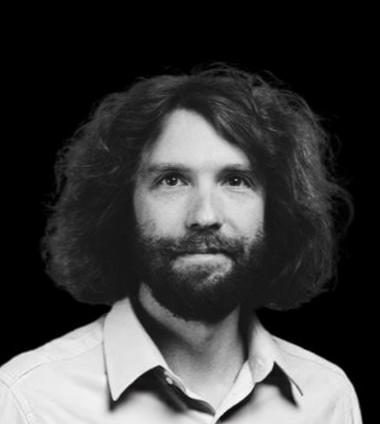
\includegraphics[width=5cm]{images/photo-thomas.png}};
\end{tikzpicture}
\end{center}
\vspace{3mm}
\begin{center}
{\displayfont\fontsize{18}{22}\selectfont\color{SEGreen}Thomas Epelbaum\par}
\vspace{1mm}
{\fontsize{9}{11}\selectfont\color{SESubtitle}\textit{SE Advisory Services}\par}
{\fontsize{9}{11}\selectfont\color{SESubtitle}\textit{PhD, CEA Saclay (IPhT)}\par}
\end{center}
\vspace{20mm}
\begin{center}
\begin{minipage}{0.75\linewidth}
\fontsize{8.5}{11}\selectfont
\noindent Thomas Epelbaum is Head of Python Developments and Machine Learning at SE Advisory Services, Schneider Electric's global consulting practice (formerly EcoAct). He built from scratch the geospatial and computational backend powering the platform's physical and transition climate risk assessments---integrating hazard projections, geolocation algorithms, and machine learning into production-grade software serving infrastructure portfolios across energy, real estate, and digital sectors. Before joining EcoAct, Thomas held data science and ML roles at Shift Technology, designing research libraries, NLP systems, and ML monitoring tools. He holds a PhD in theoretical physics from CEA Saclay (IPhT), where he studied the thermalization of the Quark-Gluon Plasma, and was trained at \'{E}cole Polytechnique and \'{E}cole Normale Sup\'{e}rieure. He brings the mathematical rigor of theoretical particle physics to climate data science and financial risk modeling.
\end{minipage}
\end{center}
\end{minipage}

\vfill